% Options for packages loaded elsewhere
\PassOptionsToPackage{unicode}{hyperref}
\PassOptionsToPackage{hyphens}{url}
\PassOptionsToPackage{dvipsnames,svgnames,x11names}{xcolor}
%
\documentclass[
  12pt]{article}

\usepackage{amsmath,amssymb}
\usepackage{iftex}
\ifPDFTeX
  \usepackage[T1]{fontenc}
  \usepackage[utf8]{inputenc}
  \usepackage{textcomp} % provide euro and other symbols
\else % if luatex or xetex
  \usepackage{unicode-math}
  \defaultfontfeatures{Scale=MatchLowercase}
  \defaultfontfeatures[\rmfamily]{Ligatures=TeX,Scale=1}
\fi
\usepackage{lmodern}
\ifPDFTeX\else  
    % xetex/luatex font selection
\fi
% Use upquote if available, for straight quotes in verbatim environments
\IfFileExists{upquote.sty}{\usepackage{upquote}}{}
\IfFileExists{microtype.sty}{% use microtype if available
  \usepackage[]{microtype}
  \UseMicrotypeSet[protrusion]{basicmath} % disable protrusion for tt fonts
}{}
\makeatletter
\@ifundefined{KOMAClassName}{% if non-KOMA class
  \IfFileExists{parskip.sty}{%
    \usepackage{parskip}
  }{% else
    \setlength{\parindent}{0pt}
    \setlength{\parskip}{6pt plus 2pt minus 1pt}}
}{% if KOMA class
  \KOMAoptions{parskip=half}}
\makeatother
\usepackage{xcolor}
\setlength{\emergencystretch}{3em} % prevent overfull lines
\setcounter{secnumdepth}{5}
% Make \paragraph and \subparagraph free-standing
\ifx\paragraph\undefined\else
  \let\oldparagraph\paragraph
  \renewcommand{\paragraph}[1]{\oldparagraph{#1}\mbox{}}
\fi
\ifx\subparagraph\undefined\else
  \let\oldsubparagraph\subparagraph
  \renewcommand{\subparagraph}[1]{\oldsubparagraph{#1}\mbox{}}
\fi


\providecommand{\tightlist}{%
  \setlength{\itemsep}{0pt}\setlength{\parskip}{0pt}}\usepackage{longtable,booktabs,array}
\usepackage{calc} % for calculating minipage widths
% Correct order of tables after \paragraph or \subparagraph
\usepackage{etoolbox}
\makeatletter
\patchcmd\longtable{\par}{\if@noskipsec\mbox{}\fi\par}{}{}
\makeatother
% Allow footnotes in longtable head/foot
\IfFileExists{footnotehyper.sty}{\usepackage{footnotehyper}}{\usepackage{footnote}}
\makesavenoteenv{longtable}
\usepackage{graphicx}
\makeatletter
\def\maxwidth{\ifdim\Gin@nat@width>\linewidth\linewidth\else\Gin@nat@width\fi}
\def\maxheight{\ifdim\Gin@nat@height>\textheight\textheight\else\Gin@nat@height\fi}
\makeatother
% Scale images if necessary, so that they will not overflow the page
% margins by default, and it is still possible to overwrite the defaults
% using explicit options in \includegraphics[width, height, ...]{}
\setkeys{Gin}{width=\maxwidth,height=\maxheight,keepaspectratio}
% Set default figure placement to htbp
\makeatletter
\def\fps@figure{htbp}
\makeatother

\addtolength{\oddsidemargin}{-.5in}%
\addtolength{\evensidemargin}{-1in}%
\addtolength{\textwidth}{1in}%
\addtolength{\textheight}{1.7in}%
\addtolength{\topmargin}{-1in}%
\usepackage{booktabs}
\usepackage{longtable}
\usepackage{array}
\usepackage{multirow}
\usepackage{wrapfig}
\usepackage{float}
\usepackage{colortbl}
\usepackage{pdflscape}
\usepackage{tabu}
\usepackage{threeparttable}
\usepackage{threeparttablex}
\usepackage[normalem]{ulem}
\usepackage{makecell}
\usepackage{xcolor}
\usepackage{amsmath}
\usepackage{float}
\usepackage{hyperref}
\usepackage[utf8]{inputenc}
\usepackage{bm}
\def\tightlist{}
\usepackage{setspace}
\newcommand\pD{$p\text{-}D$}
\newcommand\kD{$k\text{-}D$}
\newcommand\dD{$d\text{-}D$}
\makeatletter
\@ifpackageloaded{caption}{}{\usepackage{caption}}
\AtBeginDocument{%
\ifdefined\contentsname
  \renewcommand*\contentsname{Table of contents}
\else
  \newcommand\contentsname{Table of contents}
\fi
\ifdefined\listfigurename
  \renewcommand*\listfigurename{List of Figures}
\else
  \newcommand\listfigurename{List of Figures}
\fi
\ifdefined\listtablename
  \renewcommand*\listtablename{List of Tables}
\else
  \newcommand\listtablename{List of Tables}
\fi
\ifdefined\figurename
  \renewcommand*\figurename{Figure}
\else
  \newcommand\figurename{Figure}
\fi
\ifdefined\tablename
  \renewcommand*\tablename{Table}
\else
  \newcommand\tablename{Table}
\fi
}
\@ifpackageloaded{float}{}{\usepackage{float}}
\floatstyle{ruled}
\@ifundefined{c@chapter}{\newfloat{codelisting}{h}{lop}}{\newfloat{codelisting}{h}{lop}[chapter]}
\floatname{codelisting}{Listing}
\newcommand*\listoflistings{\listof{codelisting}{List of Listings}}
\makeatother
\makeatletter
\makeatother
\makeatletter
\@ifpackageloaded{caption}{}{\usepackage{caption}}
\@ifpackageloaded{subcaption}{}{\usepackage{subcaption}}
\makeatother
\ifLuaTeX
  \usepackage{selnolig}  % disable illegal ligatures
\fi
\usepackage[]{natbib}
\bibliographystyle{agsm}
\usepackage{bookmark}

\IfFileExists{xurl.sty}{\usepackage{xurl}}{} % add URL line breaks if available
\urlstyle{same} % disable monospaced font for URLs
\hypersetup{
  pdftitle={Looking at Non-Linear Dimension Reductions as Models in the Data Space},
  pdfauthor={Jayani P.G. Lakshika; Dianne Cook; Paul Harrison; Michael Lydeamore; Thiyanga S. Talagala},
  pdfkeywords={high-dimensional data, dimension reduction, hexagonal
binning, low-dimensional manifold, tour, data vizualization, model in
the data space},
  colorlinks=true,
  linkcolor={blue},
  filecolor={Maroon},
  citecolor={Blue},
  urlcolor={Blue},
  pdfcreator={LaTeX via pandoc}}


\begin{document}


\def\spacingset#1{\renewcommand{\baselinestretch}%
{#1}\small\normalsize} \spacingset{1}


%%%%%%%%%%%%%%%%%%%%%%%%%%%%%%%%%%%%%%%%%%%%%%%%%%%%%%%%%%%%%%%%%%%%%%%%%%%%%%

\title{\bf Looking at Non-Linear Dimension Reductions as Models in the
Data Space}
\author{
Jayani P.G. Lakshika\\
Econometrics \& Business Statistics, Monash University\\
and\\Dianne Cook\\
Econometrics \& Business Statistics, Monash University\\
and\\Paul Harrison\\
MGBP, BDInstitute, Monash University\\
and\\Michael Lydeamore\\
Econometrics \& Business Statistics, Monash University\\
and\\Thiyanga S. Talagala\\
Statistics, University of Sri Jayewardenepura\\
}
\maketitle

\bigskip
\bigskip
\begin{abstract}
Nonlinear dimension reduction (NLDR) techniques such as tSNE, and UMAP
provide a low-dimensional representation of high-dimensional (high-D)
data using non-linear transformation. The methods and parameter choices
can create wildly different representations, making it difficult to
decide which is best, or whether any or all are accurate or misleading.
NLDR often exaggerates random patterns, sometimes due to the samples
observed. But NLDR views have an important role in data analysis
because, if done well, they provide a concise visual (and conceptual)
summary of high-D distributions. To help evaluate the NLDR we have
developed an algorithm to show the 2D NLDR model in the high-D space,
viewed with a tour. One can see if the model fits everywhere or better
in some subspaces, or completely mismatches the data. It is used to
evaluate which 2D layout is the best representation of the high-D
distribution and see how different methods may have similar summaries or
quirks.
\end{abstract}

\noindent%
{\it Keywords:} high-dimensional data, dimension reduction, hexagonal
binning, low-dimensional manifold, tour, data vizualization, model in
the data space
\vfill

\newpage
\spacingset{1.9} % DON'T change the spacing!

\spacingset{1.0}

\section{Introduction}\label{introduction}

Non-linear dimension reduction (NLDR) is popular for making a convenient
low-dimensional (\kD{}) representation of high-dimensional (\pD{}) data.
Recently developed methods include t-distributed stochastic neighbor
embedding (tSNE) \citep{laurens2008}, uniform manifold approximation and
projection (UMAP) \citep{leland2018}, potential of heat-diffusion for
affinity-based trajectory embedding (PHATE) algorithm \citep{moon2019},
large-scale dimensionality reduction Using triplets (TriMAP)
\citep{amid2022}, and pairwise controlled manifold approximation
(PaCMAP) \citep{yingfan2021}. However, the representation generated can
vary dramatically from method to method, and with different choices of
parameters or random seeds made using the same method
(Figure~\ref{fig-NLDR-variety}). The dilemma for the analyst is then,
\textbf{which representation to use}. The choice might result in
different procedures used in the downstream analysis, or different
inferential conclusions. The research described here provides new visual
tools to aid with this decision.

\begin{figure}

\centering{

\includegraphics[width=1\textwidth,height=\textheight]{paper_files/figure-pdf/fig-NLDR-variety-1.pdf}

}

\caption{\label{fig-NLDR-variety}Six different NLDR representations of
the same data. Different techniques and different parameter choices are
used. Researchers may have seen any of these in their analysis of this
data, depending on their choice of method, or typical parameter choice.
Would they make different decisions downstream in the analysis depending
on which version seen? Which is the most accurate representation of the
structure in high dimensions?}

\end{figure}%

The paper is organised as follows. Section~\ref{sec-background} provides
a summary of the literature on NLDR, and high-dimensional data
visualization methods. Section~\ref{sec-method} contains the details of
the new methodology, including simulated data examples. Two applications
illustrating the use of the new methodology for bioinformatics and image
classification are in Section~\ref{sec-applications}. Limitations and
future directions are provided in Section~\ref{sec-discussion}.

\section{Background}\label{sec-background}

Historically, \kD{} representations of \pD{} data have been computed
using multidimensional scaling (MDS) \citep{borg2005}, which includes
principal components analysis (PCA) \citep{jolliffe2011} as a special
case. The \kD{} representation can be considered to be a layout of
points in \kD{} produced by an embedding procedure that maps the data
from \pD{}. In MDS, the \kD{} layout is constructed by minimizing a
stress function that differences distances between points in \pD{} with
potential distances between points in \kD{}. Various formulations of the
stress function result in non-metric scaling \citep{saeed2018} and
isomap \citep{silva2002}. Challenges in working with high-dimensional
data, including visualization, are outlined in \citet{johnstone2009}.

Many new methods for NLDR have emerged in recent years, all designed to
better capture specific structures potentially existing in \pD{}. Here
we focus on five currently popular techniques, tSNE, UMAP, PHATE, TriMAP
and PaCMAP. tNSE and UMAP can be considered to produce the \kD{}
minimizing the divergence between two distributions, where the
distributions are modeling the inter-point distances. PHATE, TriMAP and
PaCMAP are examples of diffusion processes \citep{coifman2005} spreading
to capture geometric shapes, that include both global and local
structure.

The array of layouts in Figure~\ref{fig-NLDR-variety} illustrate what
can emerge from the choices of method and parameters, and the random
seed that initiates the computation. Key structures interpreted from
these views suggest: (1) highly \textbf{separated clusters} (a, b, e, g,
h) with the number ranging from 3-6; (2) \textbf{stringy branches} (f),
and (3) \textbf{barely separated clusters} (c, d) which would
\textbf{contradict} the other representations.

It happens because these methods and parameter choices provide different
lenses on the interpoint distances in the data.

The alternative approach to visualizing the high-dimensional data is to
use linear projections. PCA is the classical approach, resulting in a
set of new variables which are linear combinations of the original
variables. Tours, defined by \citet{lee2021}, broaden the scope by
providing movies of linear projections, that provide views the data from
all directions. \citet{lee2021} provides an review of the main
developments in tours. There are many tour algorithms implemented, with
many available in the R package \texttt{tourr} \citep{wickham2011}, and
versions enabling better interactivity in \texttt{langevitour}
\citep{harisson2024} and \texttt{detourr} \citep{hart2022}. Linear
projections are a safe way to view high-dimensional data, because they
do not warp the space, so they are more faithful representations of the
structure. However, linear projections can be cluttered, and global
patterns can obscure local structure. The simple activity of projecting
data from \pD{} suffers from piling \citep{laa2022}, where data
concentrates in the center of projections. NLDR is designed to escape
these issues, to exaggerate structure so that it can be observed. But as
a result NLDR can hallucinate wildly, to suggest patterns that are not
actually present in the data.

The solution is to use the tour to examine how the NLDR is warping the
space. This approach follows what \citet{wickham2015} describes as
\emph{model-in-the-data-space}. The fitted model should be overlaid on
the data, to examine the fit relative the spread of the observations.
While this is straightforward, and commonly done when data is 2D, it is
also possible in \pD{}, for many models, when a tour is used.

\citet{wickham2015} provides several examples of models overlaid on the
data in \pD{}. In hierarchical clustering, a representation of the
dendrogrom using points and lines can be constructed by augmenting the
data with points marking merging of clusters. Showing the movie of
linear projections reveals shows how the algorithm sequentially fitted
the cluster model to the data. For linear discriminant analysis or
model-based clustering the model can be indicated by \((p-1)\text{-}D\)
ellipses. It is possible to see whether the elliptical shapes
appropriately matches the variance of the relevant clusters, and to
compare and contrast different fits. For PCA, one can display the \kD{}
plane of the reduced dimension using wireframes of transformed cubes.
Using a wireframe is the approach we take here, to represent the NLDR
model in \pD{}.

\section{Method}\label{sec-method}

\subsection{What is the NLDR model?}\label{what-is-the-nldr-model}

At first glance, thinking of NLDR as a modeling technique might seem
strange. It is a simplified representation or abstraction of a system,
process, or phenomenon in the real world. The \pD{} observations are the
realization of the phenomenon, and the \kD{} NLDR layout is the
simplified representation. From a statistical perspective we can
consider the distances between points in the \kD{} layout to be variance
that the model explains, and the (relative) difference with their
distances in \pD{} is the error, or unexplained variance. We can also
imagine that the positioning of points in 2D represent the fitted
values, that will have some prescribed position in \pD{} that can be
compared with their observed values. This is the conceptual framework
underlying the more formal versions of factor analysis \citep{cfa69} and
multidimensional scaling (MDS) \citep{borg2005}. (Note that, for this
thinking the full \pD{} data needs to be available, not just the
interpoint distances.)

\begin{table}

\centering{

\centering\begingroup\fontsize{12}{14}\selectfont

\begin{tabular}{>{\raggedright\arraybackslash}p{3cm}>{\raggedright\arraybackslash}p{12cm}}
\toprule
\textbf{Notation} & \textbf{Description}\\
\midrule
$n, p, k, m$ & number of observations, variables, embedding dimension, number of non-empty bins, respectively\\
$\mathbfit{X}, \mathbfit{x}$ & $p$-dimensional data (population, sample)\\
$\mathbfit{y}$ & $k$-dimensional layout\\
$P$ & orthonormal basis, generating a $d\text{-}dimensional$ linear projection of $p$-dimensional data\\
$T$ & true  model\\
\addlinespace
$g$ & functional mapping from \pD{} to \kD{}, especially as prescribed by NLDR\\
$\mathbfit{\theta}$ & (Hyper-) parameters for NLDR method\\
$r$ & ranges of the embedding components\\
$C^{(j)}$ & $j$-dimensional bin centers\\
$(b_1, b_2)$ & number of bins in each direction\\
\addlinespace
$(a_1, a_2)$ & binwidths, distance between centroids in each direction\\
$(s_1, \ s_2)$ & starting coordinates of the hexagonal grid\\
$q$ & buffer to ensure hexgrid covers data, proportion of data range, 0-1\\
$b$, $b'$ & total and non-empty hexagon bins in the grid\\
$n_k$ & number of observations within the $k^{th}$ hexagon\\
\bottomrule
\end{tabular}
\endgroup{}

}

\caption{\label{tbl-notation}Summary of notation for describing new
methodology.}

\end{table}%

We define the NLDR as a function
\(g\text{:}~ \mathbb{R}^{n\times p} \rightarrow \mathbb{R}^{n\times k}\),
with (hyper-)parameters \(\mathbfit{\theta}\). The parameters,
\(\mathbfit{\theta}\), depend on the choice of \(g\), and can be
considered part of model fitting in the traditional sense. Common
choices for \(g\) include functions used in tSNE, UMAP, PHATE, TriMAP,
PaCMAP, or MDS, although in theory any function that does this mapping
is suitable.

With our goal being to make a representation of this 2D layout that can
be lifted into high-dimensional space, the layout needs to be augmented
to include neighbour information. A simple approach would be to
triangulate the points and add edges. A more stable approach is to first
hexagonally bin the data, reducing it from \(n\) to \(m\leq n\)
observations, and connect the bin centroids. This process serves to
reduce some noisiness in the resulting surface shown in \pD{}. The steps
in this process are shown in Figure~\ref{fig-NLDR-scurve}, and
documented below.

\begin{figure}

\centering{

\includegraphics[width=1\textwidth,height=\textheight]{paper_files/figure-pdf/fig-NLDR-scurve-1.pdf}

}

\caption{\label{fig-NLDR-scurve}Key steps for constructing the model on
the UMAP layout (\(k=2\)) of the S-curve data: (a) data, (b) hexagon
bins, (c) bin centroids, and (d) triangulated centroids.}

\end{figure}%

To illustrate the method, we use \(7\text{-}D\) simulated data, which we
call the ``S-curve''. It is constructed by setting
\(X_1 = \sin(a), X_2 = U(0, 2), X_3 = \text{sign}(a) \times (\cos(a) - 1), \forall a \in [-3\pi/2, 3\pi/2]\).
The remaining variables \(X_4, X_5, X_6, X_7\) are all uniform error,
with small variance. We would consider \(T=(X_1, X_2, X_3)\) to be the
true model.

\subsubsection{Scaling the data}\label{scaling-the-data}

It is beneficial to define the algorithm on data having a standard
scale. Here the variables are scaled to {[}0, 1{]}, but the upper bound
can incorporate the aspect ratio produced by the NLDR
\((r_1, r_2, ..., r_k)\), by setting them to
\((y_{1,\text{max}}, y_{2,\text{max}}, ..., y_{k,\text{max}})\). When
\(k=2\) which is assumed for hexagon binning, \(y_{1,\text{max}}=1\) and
\(y_{2,\text{max}} = \frac{r_2}{r_1}\), as observed in
Figure~\ref{fig-NLDR-scurve}.

\subsubsection{Computing hexagon grid
configurations}\label{computing-hexagon-grid-configurations}

The 2D hexagon grid is defined by the number of bins in each direction
\((b_1, b_2)\), as given by the centroids of each hexagon \((c_1, c_2)\)
and the lower left position where the grid starts at \((s_1, s_2)\),
which correspond to the lowest left centroid. The values of \(s_i\) need
to be below their respective minimum variable values, and could be a
full bin lower, to allow a buffer (\(q\)) corresponding to a full
hexagon width (\(a_1\)) and height (\(a_2\)) around the data. The values
of \(b_i\) are variables to be computed that define the reduction in
size of the data (\(n\) to \(m\)).

The value for \(b_2\) is computed by fixing \(b_1\). Considering the
lower bound of the NLDR, \(a_1 > 2 \times s_1\), and
\(a_1 > \frac{1-s_1}{b_1 -1}\). Similarly, according to the upper bound
of the NLDR, \(a_1 > \frac{2(r_2 - s_2)}{\sqrt{3}(b_2 - 1)}\), because
\(a_2 = \frac{\sqrt(3)}{2}a_1\) for regular hexagons. Therefore,
\(b_2 = \Big\lceil1 +\frac{2(r_2 - s_2)(b_1 - 1)}{\sqrt{3}(1-s_1)}\Big\rceil\).

\begin{figure}[H]

\centering{

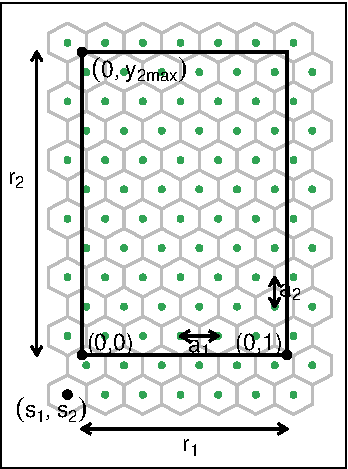
\includegraphics[width=1\textwidth,height=\textheight]{paper_files/figure-pdf/fig-hex-param-1.pdf}

}

\caption{\label{fig-hex-param}Hexagon binning parameters.}

\end{figure}%

\subsubsection{Binning the data}\label{binning-the-data}

Points are allocated to the bin they fall into based on the nearest
centroid. In situations where a point is equidistant from multiple
centroids, tie-breaking rules are applied. If multiple centroids are in
the same row, the point is assigned to the leftmost centroid. If
multiple centroids are in different rows, the point is assigned to the
bottom centroid.

\subsubsection{Obtaining bin
representations}\label{obtaining-bin-representations}

Let \(h : \mathbb{R}^{n\times k} \rightarrow \mathbb{R}^{m\times k}\) be
the function that maps a point in \kD{} space to it's bin representation
(\(C^{(k)}\)). This is the model points in \kD{} space.

When \(k = 2\), one of the representations of a bin is the hexagonal
centroid (Figure~\ref{fig-NLDR-scurve} (c)).

\subsubsection{Generating edges}\label{generating-edges}

Delaunay triangulation on bin representations generates edges by
specifying which bin representations should be connected to generate the
model in \kD{} space.

When \(k = 2\) Delaunay triangulation on \(C^{(2)}\) generates the model
in 2D space, which is a triangular mesh (Figure~\ref{fig-NLDR-scurve}
(d)). It generates convex hulls of \(C^{(2)}\) such that the
circumcircle of every triangle in the triangulation contains no other
points from \(C^{(2)}\).

\subsection{\texorpdfstring{Displaying the model in
\pD{}}{Displaying the model in }}\label{displaying-the-model-in}

The final step of the algorithm is \emph{lifting} the \kD{} model back
to \pD{}, completing the \emph{model-in-the-data-space} picture. For
this, define the set \(H^k\) to be the set of points that belong to
centroid \(k\). That is, \(H^k = \{ y \; | \; g(y) = (h_x^k, h_y^k)\}\).
We use the \pD{} Euclidean mean of the points in \(H^k\) to map the
centroid \((h_x^k, h_y^k)\) to a point in \pD{}. Let the \(i\)-th
component of the \pD{} mean be

\[f_i = \frac{1}{\left|H^k\right|}\sum_{y \in H^k} y_i,\]

with corresponding \pD{} vector \(\vec{f_i}\). Then, \(f(h\circ g)(x)\)
maps a \pD{} point to the \pD{} model estimate, completing the model
cycle.

Furthermore, edges that exist between \kD{} representations should also
generate edges in \pD{} by connecting \pD{} mapping of the corresponding
\kD{} representations.

\subsection{Measuring the fit}\label{measuring-the-fit}

\subsection{What can be learned}\label{what-can-be-learned}

\begin{itemize}
\tightlist
\item
  Overview: Generate a form that maps the model, that is the interpoint
  distances. What is the model?
\item
  Notation
\item
  Create a representation of the model

  \begin{itemize}
  \tightlist
  \item
    using hex-binning in 2D,
  \item
    parameters,
  \item
    tuning,
  \item
    pre-processing
  \end{itemize}
\item
  How does this map to the representation in high-d

  \begin{itemize}
  \tightlist
  \item
    Centroids,
  \item
    Edges
  \end{itemize}
\item
  Measuring fit

  \begin{itemize}
  \tightlist
  \item
    Fitted values
  \item
    Error calculation
  \end{itemize}
\item
  What is learned about simulated examples

  \begin{itemize}
  \tightlist
  \item
    Interesting organisation of points in UMAP
  \item
  \end{itemize}
\end{itemize}

\section{Applications}\label{sec-applications}

\subsection{pbmc}\label{pbmc}

\begin{itemize}
\tightlist
\item
  NLDR view used to illustrate clusters
\item
  Use our method to assess is it a reasonable representation
\item
  Demonstrate that it is not
\item
  Illustrate how to use our method to get a better representation
\end{itemize}

\subsection{digits: 1}\label{digits-1}

\begin{itemize}
\tightlist
\item
  NLDR is used to illustrate different ways 1's are drawn
\item
  Use our method to assess is it a reasonable representation
\item
  Demonstrate that it is, except for the anomalies
\end{itemize}

\begin{figure}[H]

\centering{

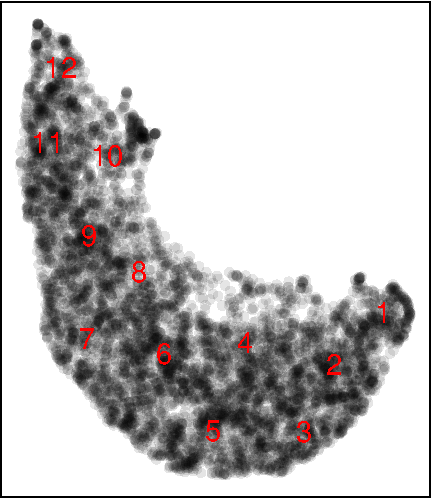
\includegraphics[width=1\textwidth,height=\textheight]{paper_files/figure-pdf/fig-pacmapauthor-1.pdf}

}

\caption{\label{fig-pacmapauthor}(a) 2D layout from PaCMAP applied for
the digit 1 of the MNIST dataset. Is this a best representation of the
original data?, and (b) Images of the handwritten digit 1. The angle of
the digit 1 varies along non-linear structure.}

\end{figure}%

\begin{figure}[H]

\centering{

\includegraphics[width=1\textwidth,height=\textheight]{paper_files/figure-pdf/fig-model-mnist-1.pdf}

}

\caption{\label{fig-model-mnist}(a) Model generated in the 2D space
overlaid on PaCMAP data, and (b) high-D model error in model space.}

\end{figure}%

\begin{figure}[H]

\centering{

\includegraphics[width=1\textwidth,height=\textheight]{paper_files/figure-pdf/fig-anomalies-1.pdf}

}

\caption{\label{fig-anomalies}(a) Images of handwritten digit 1 which
occur large model error within the non-linear strcuture, and (b) Images
of handwritten digit 1 which occur large model error outside the
non-linear structure.}

\end{figure}%

\section{Discussion}\label{sec-discussion}

\begin{itemize}
\tightlist
\item
  Summarise contributions
\item
  Explain where it is expected or not expected to work, eg higher
  dimensional relationships
\item
  Human behaviour, the desire to have more certainty, and a tendency to
  prefer the well-separated views
\item
  Predicting new observations in \(k\)-D
\item
  Extending layouts beyond \(k\)-D, when 2D is clearly inadequate.
\item
  Diagnostic app to explore differences in distances
\item
  What might be useful enhancements
\end{itemize}

\section*{References}\label{references}
\addcontentsline{toc}{section}{References}

\renewcommand{\bibsection}{}
\bibliography{bibliography.bib}

\newpage{}




\end{document}
